\documentclass[12pt,openany,a4paper]{book}
\usepackage{graphicx}	% if you want encapsulated PS figures.

% If you use a macro file called macros.tex :
% \input{macros}
% Note: The present document has its macros built in.

% Number subsections but not subsubsections:
\setcounter{secnumdepth}{2}
% Show subsections but not subsubsections in table of contents:
\setcounter{tocdepth}{2}

\pagestyle{headings}		% Chapter on left page, Section on right.
\raggedbottom

\DeclareMathSizes{12}{12}{12}{12}

\setlength{\topmargin}		{-5mm}  %  25-5 = 20mm
\setlength{\oddsidemargin}	{10mm}  % rhs page inner margin = 25+10mm
\setlength{\evensidemargin}	{0mm}   % lhs page outer margin = 25mm
\setlength{\textwidth}		{150mm} % 35 + 150 + 25 = 210mm
\setlength{\textheight}		{240mm} % 

\renewcommand{\baselinestretch}{1.2}	% Looks like 1.5 spacing.

% Stop figure/tables smaller than 3/4 page from appearing alone on a page:
\renewcommand{\textfraction}{0.25}
\renewcommand{\topfraction}{0.75}
\renewcommand{\bottomfraction}{0.75}
\renewcommand{\floatpagefraction}{0.75}

% THEOREM-LIKE ENVIRONMENTS:
\newtheorem{defn}	{Definition}	% cf. \dfn for cross-referencing
\newtheorem{theorem}	{Theorem}	% cf. \thrm for cross-referencing
\newtheorem{lemma}	{Lemma}		% cf. \lem for cross-referencing

% AIDS TO CROSS-REFERENCING (All take a label as argument):
\newcommand{\eref}[1] {(\ref{#1})}		% (...)
\newcommand{\eq}[1]   {Eq.\,(\ref{#1})}		% Eq.~(...)
\newcommand{\eqs}[2]  {Eqs.~(\ref{#1}) and~(\ref{#2})}
\newcommand{\dfn}[1]  {Definition~\ref{#1}}	% Definition~...
\newcommand{\thrm}[1] {Theorem~\ref{#1}}	% Theorem~...
\newcommand{\lem}[1]  {Lemma~\ref{#1}}		% Lemma~...
\newcommand{\fig}[1]  {Fig.\,\ref{#1}}		% Fig.~...
\newcommand{\tab}[1]  {Table~\ref{#1}}		% Table~...
\newcommand{\chap}[1] {Chapter~\ref{#1}}	% Chapter~...
\newcommand{\secn}[1] {Section~\ref{#1}}	% Section~...
\newcommand{\ssec}[1] {Subsection~\ref{#1}}	% Subsection~...

% AIDS TO FORMATTING:
\newcommand{\teq}[1]	{\mbox{$#1$}}	% in-Text EQuation (unbreakable)
\newcommand{\qed}	{\hspace*{\fill}$\bullet$}	% end of proof

% MATHEMATICAL TEMPLATES:
% Text or math mode:
\newcommand{\half}	{\ensuremath{\frac{1}{2}}}	% one-half
\newcommand{\halftxt}	{\mbox{$\frac{1}{2}$}}	  	% one-half, small
% Math mode only:
% N.B. Parentheses are ROUND; brackets are SQUARE!
\newcommand{\oneon}[1]	{\frac{1}{#1}}		  % reciprocal
\newcommand{\pow}[2]	{\left({#1}\right)^{#2}}  % Parenthesized pOWer
\newcommand{\bow}[2]	{\left[{#1}\right]^{#2}}  % Bracketed pOWer
\newcommand{\evalat}[2]	{\left.{#1}\right|_{#2}}  % EVALuated AT with bar
\newcommand{\bevalat}[2]{\left[{#1}\right]_{#2}}  % Bracketed EVALuated AT
% Total derivatives:
\newcommand{\sdd}[2]	{\frac{d{#1}}{d{#2}}}		    % Short
\newcommand{\sqdd}[2]	{\frac{d^2{#1}}{d{#2}^2}}	    % 2nd ("SQuared")
\newcommand{\ldd}[2]	{\frac{d}{d{#1}}\left({#2}\right)}  % Long paren'ed
\newcommand{\bdd}[2]	{\frac{d}{d{#2}}\left[{#2}\right]}  % long Bracketed
% Partial derivatives (same sequence as for total derivatives):
\newcommand{\sdada}[2]	{\frac{\partial {#1}}{\partial {#2}}}
\newcommand{\sqdada}[2]	{\frac{\partial ^{2}{#1}}{\partial {#2}^{2}}}
\newcommand{\ldada}[2]	{\frac{\partial}{\partial {#1}}\left({#2}\right)}
\newcommand{\bdada}[2]	{\frac{\partial}{\partial {#1}}\left[{#2}\right]}
\newcommand{\da}	{\partial}

% ORDINAL NUMBERS:
\newcommand{\ith}	{\ensuremath{i^{\rm th}}}
\newcommand{\jth}	{\ensuremath{j^{\rm th}}}
\newcommand{\kth}	{\ensuremath{k^{\rm th}}}
\newcommand{\lth}	{\ensuremath{l^{\rm th}}}
\newcommand{\mth}	{\ensuremath{m^{\rm th}}}
\newcommand{\nth}	{\ensuremath{n^{\rm th}}}

% SINUSOIDAL TIME AND SPACE-DEPENDENCY FACTORS:
\newcommand{\ejot}	{\ensuremath{e^{j\omega t}}}
\newcommand{\emjot}	{\ensuremath{e^{-j\omega t}}}

% UNITS (TEXT OR MATH MODE, WITH LEADING PADDING SPACE IF APPLICABLE):
% NB: These have not been tested since being modified for LaTeX2e.
\newcommand{\pack}	{\hspace{-0.08em}}
\newcommand{\Pack}	{\hspace{-0.12em}}
\newcommand{\mA}	{\ensuremath{\rm\,m\pack A}}
\newcommand{\dB}	{\ensuremath{\rm\,d\pack B}}
\newcommand{\dBm}	{\ensuremath{\rm\,d\pack B\pack m}}
\newcommand{\dBW}	{\ensuremath{\rm\,d\pack B\Pack W}}
\newcommand{\uF}	{\ensuremath{\rm\,\mu\pack F}}
\newcommand{\pF}	{\ensuremath{\rm\,p\pack F}}
\newcommand{\nF}	{\ensuremath{\rm\,n\pack F}}
\newcommand{\uH}	{\ensuremath{\rm\,\mu\pack H}}
\newcommand{\mH}	{\ensuremath{\rm\,m\pack H}}
\newcommand{\Hz}	{\ensuremath{\rm\,H\pack z}}
\newcommand{\kHz}	{\ensuremath{\rm\,k\pack H\pack z}}
\newcommand{\MHz}	{\ensuremath{\rm\,M\pack H\pack z}}
\newcommand{\GHz}	{\ensuremath{\rm\,G\pack H\pack z}}
\newcommand{\J}		{\ensuremath{\rm\,J}}
\newcommand{\kg}	{\ensuremath{\rm\,k\pack g}}
\newcommand{\K}		{\ensuremath{\rm\,K}}
\newcommand{\m}		{\ensuremath{\rm\,m}}
\newcommand{\cm}	{\ensuremath{\rm\,cm}}
\newcommand{\km}	{\ensuremath{\rm\,k\pack m}}
\newcommand{\mm}	{\ensuremath{\rm\,m\pack m}}
\newcommand{\nm}	{\ensuremath{\rm\,n\pack m}}
\newcommand{\um}	{\ensuremath{\rm\,\mu m}}
\newcommand{\Np}	{\ensuremath{\rm\,N\pack p}}
\newcommand{\s}		{\ensuremath{\rm\,s}}
\newcommand{\ms}	{\ensuremath{\rm\,m\pack s}}
\newcommand{\us}	{\ensuremath{\rm\,\mu s}}
\newcommand{\V}		{\ensuremath{\rm\,V}}
\newcommand{\mV}	{\ensuremath{\rm\,m\Pack V}}
\newcommand{\W}		{\ensuremath{\rm\,W}}
\newcommand{\mW}	{\ensuremath{\rm\,m\Pack W}}
\newcommand{\ohm}	{\ensuremath{\rm\,\Omega}}
\newcommand{\kohm}	{\ensuremath{\rm\,k\Omega}}
\newcommand{\Mohm}	{\ensuremath{\rm\,M\Omega}}
\newcommand{\degs}	{\ensuremath{\rm^{\circ}}}

% LaTeX run-time type-in command:
%
% \typein{Enter \protect\includeonly{...} command (or just type RETURN):}
%
% Uncommenting this command makes LaTeX prompt you for the \includeonly
% list.  At the prompt
%
%	\@typein=
%
% you type
%
%	\includeonly{chap1,chap2}
%
% to include the files chap1.tex and chap2.tex and omit any others.
% To include every \include file, just hit RETURN.
% If you are running LaTeX from xtexsh, you may need to click the mouse
% in the LaTeX window to position the cursor at the \@typein prompt.

\begin{document}

\frontmatter
% By default, frontmatter has Roman page-numbering (i,ii,...).

\begin{titlepage}
\renewcommand{\baselinestretch}{1.0}

\begin{center}

\begin{figure}
  
\includegraphics[width=\linewidth]{UQLogo.png}
\end{figure}

\vspace*{12mm}
\Huge\bf
		CONNECTING VIRTUAL ROBOTICS\\
		TO AN\\
		EXPERIMENTAL PLATFORM\\
\vspace{20mm}
\large\sl
		by\\
		Callum Rohweder
		\medskip\\
\rm
		School of Information Technology and Electrical Engineering,\\
		The University of Queensland.\\
\vspace{30mm}
		Submitted for the degree of\\
		Bachelor of Engineering
		\smallskip\\
\normalsize
		in the field of Mechatronics
		\medskip\\
\large
		June \& 2018.		
\end{center}
\end{titlepage}

\cleardoublepage

\begin{flushright}
	52 KENNIGO STREET\\
	SPRING HILL, QLD, 4000\\
	Tel.\ 0404 639 174\\
	\medskip
	\today
\end{flushright}
\begin{flushleft}
  Professor Shazia Sadiq\\
  Head of School\\
  School of Information Technology and Electrical Engineering\\
  The University of Queensland\\
  St Lucia, Q 4072\\
  \bigskip\bigskip
  Dear Professor Sadiq,
\end{flushleft}

In accordance with the requirements of the degree of Bachelor of
Engineering in the division of 
Mechatronic Engineering,
I present the
following thesis entitled `Connecting Virtual Robotics To An Experimental Platform`.  This work was performed under the supervision of Dr Surya Singh.\\

I declare that the work submitted in this thesis is my own, except as
acknowledged in the text and footnotes, and has not been previously
submitted for a degree at The University of Queensland or any other
institution.

\begin{flushright}
	Yours sincerely,\\
	\medskip

	\medskip
	Callum Rohweder.
\end{flushright}

\cleardoublepage

\chapter{Acknowledgments}

I specifically would like to thank my fellow students in the school of ITEE for assisting me during this project; for listening to the software issues I faced and giving useful insight and direction.

The product of this thesis was created in complete self-sufficiency, with functionality specified by my supervisor.

Acknowledge your supervisor, preferably with a few short and specific
statements about his/her contribution to the content and direction of
the project.  If you collaborated with another student, acknowledge
your partner's contribution, including any parts of the thesis of
which s/he was the principal author or co-author; this information can
be duplicated in footnotes to the chapters or sections to which your
partner has contributed.  Briefly describe any assistance that you
received from technical or administrative staff.  Support of family
and friends may also be acknowledged, but avoid sentimentality---or
hide it in the dedication.

\cleardoublepage

\chapter{Abstract}

% Notice that all \include files are chapters -- a logical division.
% But not all chapters are \include files; some chapters are short
% enough to be in-lined in the main file.

This document is a skeleton thesis for 4th-year students.  The
printable versions (\texttt{skel.dvi, skel.ps, skel.pdf})
show the structure of a typical thesis with some notes on the content
and purpose of each part.  The notes are meant to be informative but
not necessarily illustrative; for example, this paragraph is not
really an abstract, because it contains information not found
elsewhere in the document.  The \LaTeXe\ source file
(\texttt{skel.tex}) contains some non-printing comments giving
additional information for students who wish to typeset their theses
in \LaTeX.  You can download the source, edit out the unwanted
material, insert your own frontmatter and bibliographic entries, and
in-line or \verb+\include{}+ your own chapter files.  Of course the
content of a particular thesis will influence the form to a large
extent.  Hence this document should not be seen as an attempt to force
every thesis into the same mold.  If in doubt about the structure of
your thesis, seek advice from your supervisor.

\tableofcontents

\listoffigures
\addcontentsline{toc}{chapter}{List of Figures}

\listoftables
\addcontentsline{toc}{chapter}{List of Tables}

% If file los.tex begins with ``\chapter{List of Symbols}'':
% \include{los}

\cleardoublepage

\mainmatter
% By default, mainmatter has Arabic page-numbering (1,2,...).


% Chapters may be \include files, each beginning with a line like
%
%	\chapter{Title of chapter}
%
% e.g. if two chapter files were called intro.tex and theory.tex,
% we would say
%
%	\include{intro}
%	\include{theory}

\chapter{Introduction}
%% Introduction of thesis problem and thesis
Remotely controlling a robot or robotic manipulator is a desirable objective with large complications to still be overcome. It is proposed that doing this through a virtual environment can eliminate collisions or undesirable actions that may incidentally occur due to the nature of long distance control, whilst providing the benefits of virtual simulations. Specifically, this thesis focuses on the development a remote interface to a 'Virtual Robotics Environment Platform', VREP. VREP can be used to simulate robotic arms and processes, and includes the commonly used wheel-chair based Kinova Jaco arm which is available at the University of Queensland. The remote interface, otherwise known as the 'client program' (given that it treats VREP as the server), was designed to take input from a user by either keyboard or joystick, and have the motion played out in VREP, corrected for any obstructions, and then control the movement of the Jaco arm through the Kinova Software Development Kit.

%% Introduction to virtual simuations
In all engineering disciplines, virtual simulations allow one to view and interact with an environment or process in a non-destructive manner. Simulations can provide a realistic rendering of an event, whilst providing further detail into physical phenomena that establish design constraints, and optimization techniques. Robotics makes use of lumped electromechanical components to interact with an environment in a desirable manner. Thus, virtual robotics is a necessary field for growth in engineering, as it allows the testing of interactions with an environment whilst giving unforeseen insight.

%% Introduction to robotics
Companies such as those in manufacturing, technical experts in the fields of medicine and surgery, and persons with disabilities all benefit from the capability of robotic manipulators. In most circumstances it is expected that these manipulators can be controlled by a user in real time, however this ability is restricted by inherent delay in the process of receiving an input, calculating an action, and actuating. Further expectations of robotics include optimality and customisation; where it may be desirable for movements of a robot to minimize the energy used in a given process or a robotic arm to pick up a glass a in a certain manner. This provides interconnected layers of desired functionality for a robot; a layer dedicated to moving the manipulator, a layer designed to create movements that meet the user's needs whilst minimizing design criteria, and a monitoring layer that focuses on aspects such as physical constraints and robotic learning.

%% Introduction to remote robotics
With the invention of the internet to provide long range data-resourcing, came a desire to move the control of manipulators and processes to a remote location. The concept of remote robotics is no different to the typical method of controlling manipulators, an input has a desired output, however at some time in between, data is processed and sent through the internet. Given factors such as time to send, packet loss, processing time, and internet traffic, a significant amount of undesirable delay is added and decreases the satisfaction of real-time control. This produces large complications in areas such as remote robotic surgery, where reaction delay may have harmful effects.

%% Introduction to thesis hypothesis
Virtual robotic environments can simulate the true movements of a manipulator given its physical attributes. VREP in particular can calculate the joint angles required to be able to move the hand from one position to another using a physics engine and accuracy of choice. It is believed that allowing a virtual environment to compute the movements required by a remote user will increase the accuracy in movement and decrease the chance of collision of the physical robot.

%% Introduction to thesis scope
Although this thesis does not go into large detail on the testing of the complete product, remote user to physical robotic arm movement, it does go through the design of the remote interface. The problems faced in controlling a robotic arm, design strategies tested, and the future improvements of the client program are presented. This interface was crucial to the success of the whole system, and it was important to refine before interfacing with a physical arm. Included in this document is:

\begin{itemize}
	\item A comparison of different approaches for moving a robotic arm, along with the calculations and methods for refining accuracy and decreasing processing time.
	\item An overview of VREP, and how its features were used to replicate the true movements of the Jaco arm. This includes a comparison of the available physics engines, the use of PID motor control for arm joints and Inverse Kinematics (IK) functionality. 
	\item Validity of using VREP as a real-time simulation tool, looking into aspects such as rendering delay and communication techniques.
	\item The features included in client program and how its functionality was shaped, and the limitations associated with a real-time program performing large amounts of calculations based off user inputs and a remote server.
	\item An overview of the Jaco Kinova arm and it's software development kit, which can be used to control the Jaco arm from VREP or the client program.


\end{itemize}
% list scope


%% Introduction to thesis objectives
To accomplish the task of remotely controlling the Jaco arm with collision avoidance, the project was broken into four main stages. The long-term objectives to acheive the aforementioned goals, presented in \label{Original Objectives}, are:

\begin{itemize}
	\item to configure the external simulation control of VREP and the Jaco arm within. This included retrieving all of the arm's joint information on start-up, so the correct joints can be referenced during connection. The central purpose of this objective was to achieve control of the arm in simulation, getting it to move its gripper to desired coordinates.
	\item using the information from VREP of the arm, and the current joint angles from the physical Jaco arm using the SDK, achieve movement replication between the the physical and virtual systems. The purpose of this was that it would allow tuning of the VREP simulation to mimic the way the physical arm moves and responds to commands.
	\item with VREP tuned appropriately, allow the movement of the physical arm by controlling movement in the simulation. It was predicted that movement in the simulation would come from keyboard commands or on-screen mouse presses.
	\item detect collision, move objects in the laboratory and interact with the environment in simulation, with the Jaco arm replicating the motion.

\end{itemize}


Due to unforeseen circumstances, the objectives presented in this project changed to focus on the different ways of interacting with the virtual arm through VREP's remote API. It's primary focus is the validity of using a remote client to interact with VREP, and whether a good interface with the aforementioned requirements can be created. The objectives of this thesis were to:

\begin{itemize}
	\item Create a user friendly interface for controlling a robotic arm in VREP, robust to arm location within a scene and mode of the virtual arm (forward kinematics or inverse kinematics modes)
	\item Allow the user to give input types as they desire, such as moving the Jaco arm gripper from point to point, or controlling the joint angles individually; with keyboard input or joystick input.
	\item Experiment with different mathematical solutions and physics engines to achieve accurate and fast movement of the virtual robotic arm
	\item Experiment and outline the different functionality VREP has to offer, which may be utilised in the development of the over-arching objectives.
\end{itemize}

The required functionality of this project can be seen in the figure below. A user controls the VREP client program, which communicates with the virtual robotic arm for the interest of collision avoidance. From this, the client program can interface with the program designed to communicate with the Kinova API to control the physical arm. The movements of the physical arm are a mimic of the virtual arm's movements without collisions.


\begin{center}
\begin{figure}[htb]
  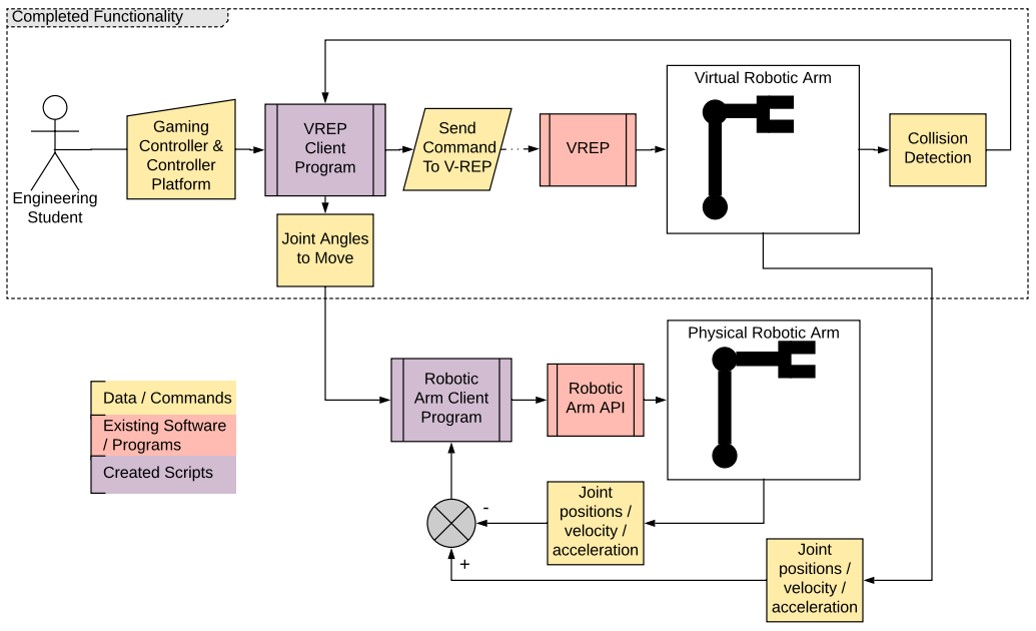
\includegraphics[width=1.12\linewidth]{Thesis_flow_chart.jpg}
\caption{Flow diagram describing the key features of this thesis}
\end{figure}
\end{center}


% leading introduction statement
From here, a variety of challenges will be pondered as mathematical formulas are derived to describe the motion of a 6 degree of freedom (DOF) arm, and a remote interface is created for allowing real-time movement within VREP.\\

%% default intro
%The introductory chapter describes the importance of the field and the
%scope and significance of your project.  It usually ends with an
%overview of the remainder of the thesis.%
%
%Notice that Arabic page numbering begins with Chapter 1.  Preceding
%pages (known as ``frontmatter'') have Roman numbering.  The
%\texttt{book} document class in \LaTeX\ follows this numbering
%convention by default (see Lamport~\cite{lamport}, p.\,80).
%%
%%\chapter{Literature review / prior art}
%
%You will need to review previous work in the field, which may include
%books and papers (``literature''), patents and commercial products
%(``prior art''), and earlier work in your Department.  This
%information is usually (but not always) collected in a single chapter,
%whose title should preferably be more specific and interesting than
%the one above.
\chapter{Programming Robots to Move}
%% Go through case studies of how robots have been programmed to move in the past
In order to move a robotic arm, two layers of control are required, the motor position control for each joint, and the system that depicts how much the joints need to change angle when moving from one arm configuration to another. Following are some case studies that present methods of controlling a robotic arm, where the maths behind them are left for the theory section of this report.

\section{MATLAB Toolboxes}
Matlab provides an extraordinary amount of support for calculating the important properties required for the control of a robotic manipulator. Below is a sample of some of the useful libraries available that were, and further could be, beneficial to creating an interface for controlling the virtual Kinova Jaco arm remotely.

\subsection{Robotics Toolbox}
%https://robotacademy.net.au/masterclass/inverse-kinematics-and-robot-motion/?lesson=301
Professor Peter Corke, the Director of the Australian Centre for Robotic Vision (ACRV), has designed a Matlab specific toolbox for computing the mechanics associated with robotic manipulators. Included is easy to use functions for creating robotic arms, and calculating parameters such as forward and inverse kinematics, trajectory generation and control systems for motor control. Within the Queensland University of Technology's Robot Academy is 'Master Classes' on using the toolbox through examples of simple manipulators and the theory behind the complex calculus being performed.\\

There are dozens of object files containing the parameters of robotic manipulators; including the 6 DOF puma560 and limited information on the 6DOF Kinova Jaco arm. The parameters within these files contain the link times of the arm, the Denavit-Hartenberg parameters (DH parameters - theory section of this report), and can contain inertial and angle properties for each link. These properties are helpful in computing the forward kinematics, inverse kinematics, and dynamic equation representing the motion and torques on the arm.

With this, the toolbox allows the viewing of the manipulator in desired angles, the movement of the arm between two desired end-effector positions, and the building of the control system controlling the torque at each motor given the current arm configuration. The latter of which is crucially important in providing accurate control of the arm, in ensuring the appropriate power is provided to all of the joint links as it moves over a given trajectory. Unfortunately, it is extremely difficult to compute, and for each degree of freedom contains 10 constants that need finding; mostly inertia terms which for each link depends on its orientation and position relative to the arm's base; thus relying on all link angles between the base and the link of interest. The mechanics of this is presented in the theory section of the report, but the Robotics Toolbox provides functions which compute the inertial, coriolis and gravitational torques acting on the arm. Professor Corke also provides a method of motor control for each link given the aforementioned parameters are known. The method uses the typical motor position control strategy of a Proportional Derivative Controller (details in the theory section) to compute the required motor torque from the error in angle position and velocity, however also includes a feed-forward component of the calculated disturbance torque due to the coupled dynamics between links. 

\begin{center}
\begin{figure}[htb]
  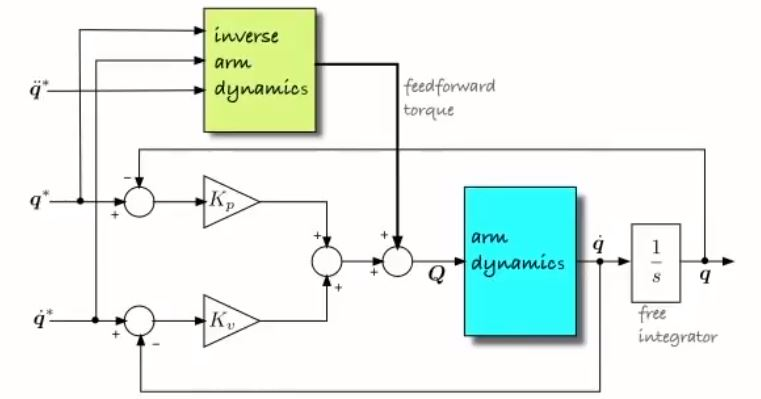
\includegraphics[width=\linewidth]{Correcting_for_disturbance_torque.jpg}
\caption{Motor Torque Control System}
\end{figure}
\end{center}

Thus the torque provided at each link can be expressed as:

$\tau = K_p (q^{*} - q) + K_v (\dot{q^{*}} - \dot{q}) + M(q) \ddot{q^{*}} + C_j (q, \dot{q}) \dot{q} + g_j (q)$

Where the change in angle required by each joint when moving the end-effector from one coordinate to another can be computed using the variation of the 'ikine' function for the given robotic arm; the forward kinematics can be computed similarly using the 'fkine' function.
%% this should be compared to how VREP controls the arm using PID in the theory section. Additionally, the advantage of calculating the dynamic equation for the arm for LQR

\subsection{Robotic Arm Models}
%https://au.mathworks.com/help/physmod/sm/ug/import-robot-arm-model.html
%https://au.mathworks.com/help/control/examples/multi-loop-pid-control-of-a-robot-arm.html?searchHighlight=robotic%20arm&s_tid=doc_srchtitle
Separate to the custom designed toolbox of Professor Corke, MATLAB has its own robot manipulator modelling sub-program and alternative methods of control. Simscape allows the creation of physical systems within MATLAB's simulation tool Simulink. An example of 6 DOF robotic arm is presented below; the base of the arm represents the origin, and the lines span out from this with rigid bodies followed by links. Each rigid body can be shaped within MATLAB or imported from a CAD model to produce a replica of the real robotic arm; where properties such as material and interia can be defined.

\begin{center}
\begin{figure}[htb]
  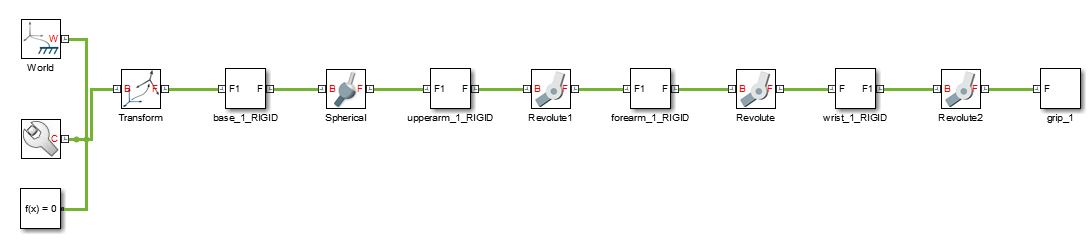
\includegraphics[width=\linewidth]{simscape_robotic_arm.jpg}
\caption{smrobot Simscape Model}
\end{figure}
\end{center}

Simulating the model shown above will provide a visualisation of the arms and any motion set on it by external forces or motor torques; not included in the above model.

\begin{center}
\begin{figure}[htb]
  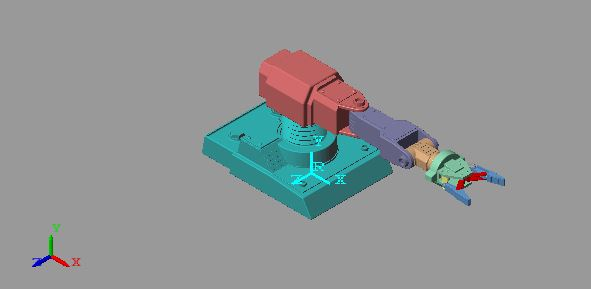
\includegraphics[width=\linewidth]{simscape_robotic_arm_model.jpg}
\caption{smrobot Simscape Model Visualisation}
\end{figure}
\end{center}

From here, it is a matter of controlling the robotic arm to move from one joint configuration to another. For a custom robotic arm, any of the strategies outlined in the theory section of this report can be used, however MATLAB provides another means which is described in the section below. In order to move the joints from one position to the next, a strategy similar to that shown in Figure 2.1 is required. In simulink, the layer of controlling the motor position can be formatted as follows:

\begin{center}
\begin{figure}[htb]
  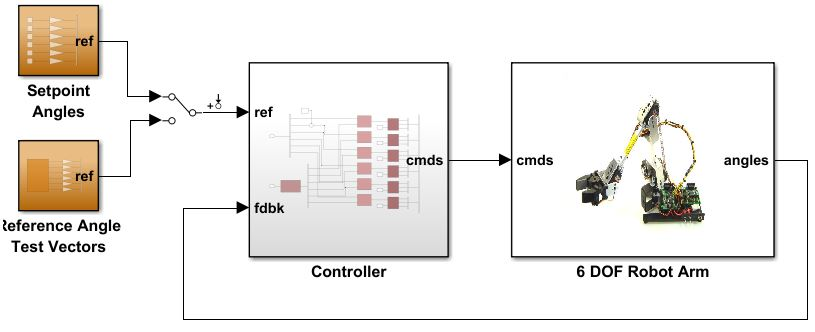
\includegraphics[width=\linewidth]{simulink_motor_control_loop.jpg}
\caption{Simulink Model of Motor Control Loop}
\end{figure}
\end{center}

Where nested within the controller is the tuned PID controllers for each motor which drives it to the desired position. This is similar to Peter Corke's method but without pre-emptive knowledge of the disturbance torque due to the arm's dynamic coupling.

\begin{center}
\begin{figure}[htb]
  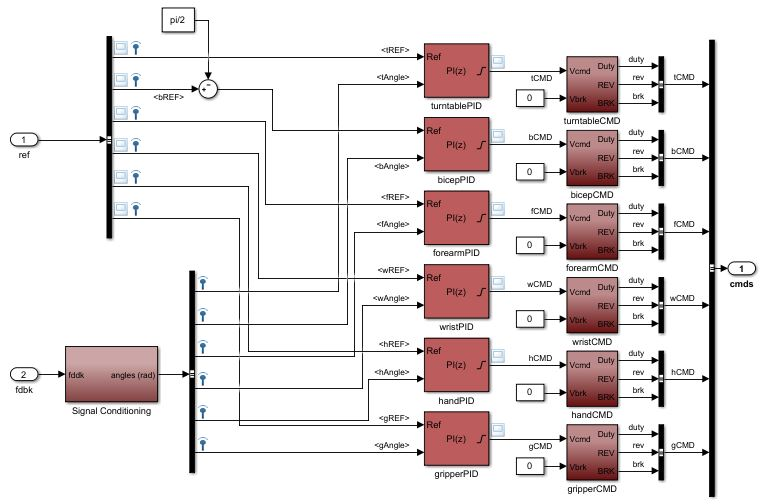
\includegraphics[width=\linewidth]{simulink_motor_control_PID.jpg}
\caption{Simulink Model of Motor Controllers}
\end{figure}
\end{center}

It will be seen that VREP operates in the same way, as it enables the importing of manipulator models and setting of each joint's controller coefficients. The figure above gives a good representation of the mechanics behind what the parameters are doing in terms of regulating each joint's error to a desired angle. A significant advantage of MATLAB is the auto-tuning functionality of the PID controllers for each joint, however a controller on it's own would not be as robust as that described in the Robotics Toolbox section.

\subsection{Adaptive Neuro-Fuzzy Inference System}
%https://au.mathworks.com/help/fuzzy/modeling-inverse-kinematics-in-a-robotic-arm.html?searchHighlight=robotic%20arm&s_tid=doc_srchtitle
An Adaptive Neuro-Fuzzy Inference System (ANFIS) network can be used to deduce the joint angles required for an arm's end-effector to reach a desired 3-D position. Calculating the required angles analytically for an arm of greater than 4 DOF can become challenging and result in infinitely many solutions. Like any neural network, with a sufficiently large dataset the internal weights will learn what angles will result in the desired end-effector position. Thus, in training an ANFIS to control each joint for a training dataset, it is able to interpolate angles to sufficient accuracy and move the joints to reach a desired end-effector position.

To train the network, input to output mapping data is required. Thus, given the forward kinematics for a robotic manipulator is known, a dataset of angles to end-effector position can be created over the space that it is desired for the end-effector to move. After the network gains its own understanding of the mapping, any point within the testing region can be given and the network return the required joint angles. In a MATLAB example, each joint is given its own network to be trained such that for each joint an angle will be provided given a desired position. Outside the range of training, the manipulator will not respond promisingly, and thus for a large control range, a sufficiently large dataset is required. Overall neural networks respond quickly to providing results once trained, however the training process can be time consuming.

\section{Programmed Robotic Arms}
%https://pdfs.semanticscholar.org/75f2/fa10a66e35bd6b5b5d695b31be51df78303e.pdf
Volume 58 of the 2012 International Journal of Computer Applications, titled Software Development for an Inverse Kinematics of Seven-Degrees of Freedon Newly Designed Articulated Inspection Robot, details on previous software development tools used to control robotic manipulators. It is detailed that the inverse kinematics can be solved using an Adaptive Neuro Fuzzy Network (ANFIS), a neural network trained to reduce error in end effector position, non-linear optimization methods, geometric approaches, and through the manipulation of the transformation matrices. In the ANFIS approach, it was noted that MATLAB was used, however C / C++ programming has been used to develop programs that compute the more mathematics based inverse kinematics methods. A program is proposed in this paper which uses Visual-Basic to allow the calculation of forward and inverse kinematics, and trajectory planning.\\



%http://scholarcommons.usf.edu/cgi/viewcontent.cgi?article=2791&context=etd
A thesis paper from the University of South Florida comments on the fact that programming in a low level language such as C is closer to the hardware level which reduces computation time in processing and communicating with external systems (sensors and motors). High-level languages, such as MATLAB, provide an user-friendly interface for solving complex maths operations, however lack capabilities found in C / C++ such has multi-threading and easy communication between concurrently running processes. It is explained that the complexity in configuring MATLAB to communicate with a separate C++ program lead to failure of the wheel-chair mounted robotic arm's program on multiple occasions. The software system in this paper refers to using a C++ program used to communicate with sensors and other hardware, whilst using MATLAB for the control algorithm computations, and simulation. Due to the aforementioned advantages of C++, a new C++ program, with an external library for matrix manipulation, was created to replace the MATLAB program. The concluding results being that the new software system reduced delays in the control of the robotic arm, leading to better stability and control.\\
The primary purpose of using MATLAB in this experiment was to simulate a virtual model of the robotic arm, and using the angles of this to control the physical robotic arm through the C++ platform. The complexity and delay produced by MATLAB lead to slow and unreliable control.\\



The Kinova Jaco arm's Software Development Kit (SDK) is written in C++, with the handling of communication and calculations stored in an human-unreadable dynamic link library. There is no documentation into how the SDK calculates the joint angles required for a desired gripper position, however there are usage examples in C++ of all the available functions; one of which is used to setting the gripper position and angle in cartesian coordinates. This SDK allows direct tuning of crucial arm parameters such as maximum applied torque, PID coefficients and velocity control. Predefined structures can be filled with this information and sent to the arm's FIFO buffer to interpret and act accordingly, making the control of the arm from the developer's perspective effortless.\\
Controlling the robotic arm in this way however, means the arm needs to be completely set-up in order to use the SDK. It may also be hard to understand how the parameters affect the movement of the arm; for example, the coordinate system isn't well defined and will take some trial and error to understand. This could be done with the help of the `get` functions, which can return torque, velocity and position values of the arms current configuration. To further understand how the settings can affect the arm, Kinova have supplied the `Development Center` with the SDK (which back-end C++ code is accessible, and can provide knowledge into how the arm can be controlled) what allows the user to move the arm, set trajectories, and review current parameters.\\



% I really don't know much about ROS... RVIZ?
%http://wiki.ros.org/ROS/Introduction
%https://github.com/Kinovarobotics/kinova-ros
The Robot Operating System (ROS) is a modular collection of commonly used software in low-level device control, hardware abstraction and functionality seen in robotics. ROS can be used in Python, C++ and Lisp programming languages to build a framework around robotic software kits that directly control a robotic actuator. Thus, it has already been used as a cover of the Kinova SDK for the Jaco arm. Further, simulation platforms such as Gazebo and MoveIt can be controlled using ROS, with the software for controlling a Jaco arm in Gazebo being available. Together, ROS can be used to control a virtual model of the Jaco arm in Gazebo, as well as the physical arm through the Kinova SDK. Control of robotic manipulators in VREP is also available using ROS through the VREP remote API.\\
%https://pdfs.semanticscholar.org/2600/e3b018b5fa77035dab558f783919c9d46d35.pdf
ROS offers a package called Rvis, which provides a method of interacting with imported models in 3D. Similar to a robotics simulation package, Rvis can provide information about the centre of mass of objects, collisions, and joints of robotic manipulators and objects in a scene. It however lacks the real-world modelling that comes with simulation programs such as V-REP or Gazebo (running a physics engine). Thus, it is typically used as a wrapper for these programs, such that the user can retrieve key information about objects in a scene whilst simulating properties such as gravity and friction.


%https://robotacademy.net.au/lesson/inverting-the-jacobian-matrix-2/
In Professor Peter Corke's Robot Academy series, he goes through an intuitive explanation for programming robotic arms using the arm's Jacobian matrix (referenced in Theory). As the Jacobian is a function of joint angles, it only provides a truthful reflection of the small change in angles required for a small change in end effector position, local to the current arm configuration. Thus, the Jacobian matrix can give a solution for small angle changes, but after the arm moves to this new position, it must be recalculated. This can be done in programming using discrete time steps as outlined in the figure below. Unfortunately, as this is an approximation technique, if any of the spacial or time parameters are too large, the result will no longer hold, and thus it should be used with caution.

\begin{center}
\begin{figure}[htb]
  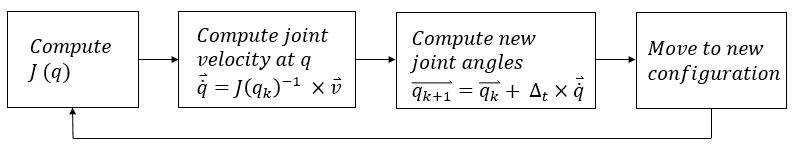
\includegraphics[width=\linewidth]{jacobian_programming.jpg}
\caption{Flow Diagram of using Jacobian in Programming}
\end{figure}
\end{center}

A similar technique that can reduce the error between the end effector's position and a small change in position is the PID controller. With the appropriate weightings for each joint, the joints can be moved to reduce the error in end effector position. Note that there is no control of the joint-space in this case, and could lead to undesired joint configurations. This gives the Jacobian an advantage, as it is non-invertible at a joint singularity; when the arm looses a degree of freedom.


\section{Simulation Platforms and Physics Engines}
%https://www.smashingrobotics.com/most-advanced-and-used-robotics-simulation-software/
There are numerous platforms available for simulating the dynamics and interactions of robot's with a scene. V-REP is particularly useful for this thesis due to its ability to remotely control the simulation and the objects within, whilst providing a realistic environment for said interactions. Other popular robotic platforms have similar functionality, but may come at a cost, include Webots, Robot Studio, ARGoS, labVIEW, Visual Components, Virtual Robotics Toolkit, Gazebo, Actin Simulation and Workspace. Although the objective of these platforms is to simulate a robotic manipulator in a scene, they are customized in the robots that can be simulated, the physics engine they use to simulate the dynamics, and the requirements by the users using the product. A good example of this is the Robot Virtual Worlds platform, which has comprehensive capabilities in simulating and programming LEGO robotics. On the contary, Workspace is used for simulating industrial production lines with multiple robotic manipulators acting together; and is used by large companies such as ABB and Mitsubishi. The scope of this thesis focuses on the use of free simulators that provide realistic and programmable simulations for educational use. Thus, simulation platforms such as Webots, Gazebo and V-REP are of particular interest as they equally provide the required features to meet the objectives. 

%https://arxiv.org/pdf/1402.7050.pdf
An online survey was conducted by researchers Serena Ivaldi, Vincent Padois and Franceso Nori to determine which simulation platform and dynamics solver was most preferred. The survey was completed by 119 participants with 62\% possessing a PhD, and of the remaining, 32\% had a university level degree. It was found that 39\% of the participants hadn't heard of V-REP, compared to 27\% and 15\% for Webots and Gazebo respectively. However, it was found that V-REP was the best rated for usability, documentation and set-up guides, whereas Gazebo was the most used. From the findings, it was noted that V-REP was the most likely for applicants to try, and keep using, compared to Webots and Gazebo.

%http://www.dca.fee.unicamp.br/~gudwin/courses/IA889/2014/IA889-02.pdf
A full comparison between Gazebo and V-REP was conducted by Lucas Noguira from the Universidade de Campinas. This article goes through implementing features common to both platforms and the process required for setting them up to do a given task; i.e. connect a sensor to a robot and read it through ROS. It was found that V-REP offered a much better interface for adding components, and used less computation time when compared. 

\subsection{V-REP}
% Introduce V-REP
The robotics simulation platform used in this thesis is the Virtual Robotics Experimental Platform (V-REP) by Coppelia Robotics. V-REP offers a means of realistically simulating mobile robotics and actuators with an easy to use interface. In a simulation, V-REP continuously reads an internal `main` Lua script, that may read other scripts describing properties associated with robotics in the scene, which are customisable by the user. On the side pane is a large list of available robots that can be imported, and once they are, a script customised by Coppelia is loaded to the list of running scripts; i.e. in the case of the Jaco arm, a script is imported that moves the arm around in the scene to a pre-configured trajectory. The simulation process is described by the figure below, where it can be seen that the main flow of code goes between actuation, reaction, sensing and control, with monitoring collisions being the main priority at each stage.

\begin{center}
\begin{figure}[htb]
  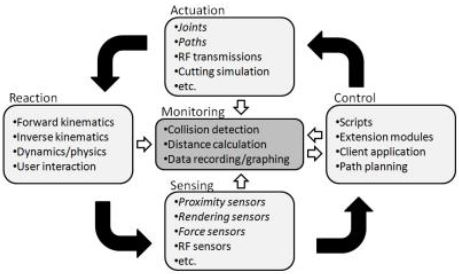
\includegraphics[width=\linewidth]{vrep_simulation_diagram.jpg}
\caption{Flow Diagram of the V-REP Simulation}
\end{figure}
\end{center}

\subsubsection{Communication}
%Introduce a means of communicating with V-REP
%http://www.coppeliarobotics.com/helpFiles/en/writingCode.htm#sixMethods
Fortunately, the parameters within these scripts and objects within the scene can be controlled using the remote API, which is available for C/C++, Python, Java, Matlab, Octava, Lua and Urbi. The documentation for the remote API contains extensive descriptions of over 100 functions, where the usage is available for all supported languages. Additionally to the remote API and internal Lua scripts, there are 4 other methods of controlling a scene in V-REP. The most obvious is plugins, which can provide custom Lua commands for interacting with the internal Lua scripts, it is effectively an external library of functions. Similarly, ROS can provide a wrapper of V-REP, enabling control from any ROS supported coding language, and further can enable the control of an external robot through a ROS node, using the information from V-REP; which is the aim of this thesis to a large extent. ROS. There is no limitations to utilizing V-REP's capabilities between using a remote API client and a ROS node, as seen in the connection methods table on the V-REP website; both will contain lag due to communication over the internet through a socket connection. Other methods of controlling V-REP include through the use of an add-on, or a BlueZero node.

%Introduce the methods of communication with V-REP remote API
Communication using the remote API is through a socket connection between the client API and VREP. To enable connection, V-REP needs to be configured to allow external connections through a specified port; there is no restriction to the number of open ports, however it does induce simulation lag. As scripts are associated with objects within the scene, this configuration is typically set in a threaded child script of an invisible dummy object in the V-REP scene; an example of this can be seen below. 

\begin{center}
\begin{figure}[htb]
  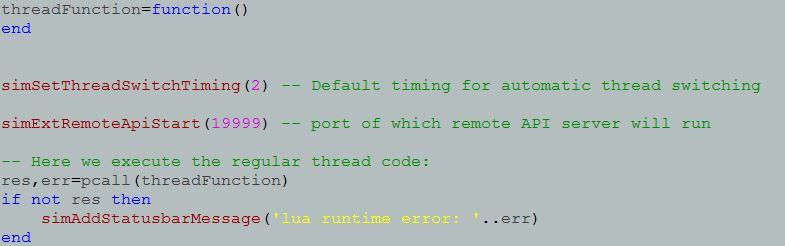
\includegraphics[width=\linewidth]{vrep_port_listen.jpg}
\caption{Sample Lua Code for Connecting V-REP to a port}
\end{figure}
\end{center}
%http://www.coppeliarobotics.com/helpFiles/en/remoteApiFunctions.htm
On the client side, connecting to V-REP waits for a given length of time for a client identification number. Once this number is obtained, the number is used for all communication thereafter in a manner noted by Coppelia for the language chosen. As an example, the functions could return parameters such as joint angles, velocity and sensor outputs, alternatively the functions could also be used to set or change these parameters.
% need to discuss at some stage that communication isn't guaranteed between different networks, i.e. home verse uni

Communication between the client program and V-REP is undertaken in four different modes; blocking function calls, non-blocking function calls, data streaming and synchronous operation.

\begin{center}
\begin{table}[htb]


    \begin{tabular}{ | l | p{10cm} |}
    \hline
    Operation Mode & Summary \\ \hline
     Blocking & When a command is sent in blocking mode, the client will wait until the V-REP API response before moving to the next line of code.\\ \hline
    Non-blocking & When data needs to be updated in the client program, that isn't required straight away. The client can make a call for the data to be copied to a particular address and move on to the next line. The API will respond in due time.  \\ \hline
    Data Streaming & When the same data is constantly required from V-REP, the data-streaming method allows a way for V-REP to send updates of a particular value without calling for it each time. For instance, joint angles of a robotic arm may be required by the client program with large frequency, and could be updated without making direct calls and waiting for a response each time once a data-streaming call is given. This is a continuous mode, and the client will be stuck receiving data. \\
    \hline
    Synchronous & When it is desired to have the simulation and client program run concurrently in time, such that the simulation advances with the client. Synchronous mode allows the client to control the advancement of the simulation.\\
    \hline
    \end{tabular}
    \caption{V-REP remote API operation modes}
\end{table}
\end{center}

To be able to interact with a particular object in V-REP, one must refer to it in function calls using its `object handle`. The object handle is a unique number given to every object in a scene, typically in order of when the object was added to the scene, known by its appearance in the scene hierarchy; a list containing all of the objects in the scene, starting with objects like the default camera, floor, lights, XYZ coordinate frame, and then any objects that were placed in the scene after. Once an object has been deleted from the middle of the hierarchy, the other objects retain their object handle; thus once an item is added its object handle won't change. When calling a missing object in a scene, NULL will be returned.

\subsubsection{V-REP Features}

Models can be imported into V-REP as a mesh (.stl) from any 3D modelling software (such as AutoDesk). The models can either be static objects to be placed in the scene, or make up parts of a robotic manipulator. When importing models, it is important to consider the amount of triangles used to create the component, when this is too large (more than 20,000), manipulating the object in V-REP will come with noticeable lag. When building a robotic arm from a CAD drawing, the entire model can be imported, and then subdivided to form an interaction `group` of meshes. When the Denavit-Hartenberg parameters of the arm are known, these can be used to form the relationship between the joints. The interactions between parts can be made by adding translational and/or rotational relationships, with parameters such as maximum angle and starting position specified. All of the objects in the scene can be modified out of simulation to be dynamic or static (be influenced by external forces), and responsive or non-responsive (have a reaction when a collision with the object occurs). It should be noted that the object doesn't need to be part of a robot, but can be an object in the scene either as a feature or an interactable object.\\


On start-up, V-REP comes with 21 pre-assembled non-mobile robotic manipulators (arms), including the Kinova Jaco and Mico arms. Other V-REP supported models can be loaded into a scene, given the appropriate .ttm format. The model browser also includes a selection of pre-made models, such as arm grippers, sensors, furniture, household appliances, people, vehicles and mobile robots. Using the model browser alone, it is possible to replicate a room or scene that a real robot would interact with. The robots can also be placed on any surface in the scene, and be provided a given trajectory or motion path for interacting with objects.\\


Collision detection is an important feature required for this thesis, as the objective is to detect collisions within the scene. V-REP has a collision detection feature, which will register collisions between collidable entity-pairs. Thus, objects that may collide within a scene need to be set prior to simulation; a robotic arm can be set to 'Enable all collision detections', which will flag when the robotic arm collides with any object. From a remote API client's prospective, this isn't yet helpful as V-REP will not flag a collision to the client automatically. Instead, the client program will need to ask for the execution of a custom Lua function within V-REP, which will use the simCheckCollision function to check for collisions within the scene, and then stream the response back to the client. Thus, this could be used in a data-streaming method, where the client is continuously checking for data from V-REP being send from the custom function. Alternatively, the remote API contains a simxReadCollision function which can be called given an object's collision handle (i.e. a link of a robotic arm pre-registered to potentially collide), where the response will indicate a collision or lack there of.\\


%% need to go into the inverse - forwards kinematics... Still not sure how they solve for these given any model can be created in V-REP...
The most useful feature of V-REP's for this thesis is the kinematics solver, where the arm can be set to either forward kinematics or inverse kinematics mode. By default, one is able to give joints desired positions, and the PID controller representing the motor dynamics actuates the joint to produce a realistic resulting position at that of which is desired; unless the motor actuation saturates, resulting in steady-state error from the goal position. From the V-REP client, one is able to send desired position, velocity and actuation force to the joints of a robotic manipulator at any given moment. Conversely, when the position of a joint in space is desired, the calculation of the angles to produce this goal position is required. V-REP is able to solve this inverse kinematics problem, given a desired position, the links requiring moving and the joint position to be moved are known; and the desired position is in reach of the arm, i.e. the solution is solvable.\\
To set a robotic arm to inverse kinematics mode such that the end-effector reaches a goal position, a dummy object representing the `Target` for the gripper must be added. It may be desirable to also create a `Tip` dummy object that moves with the gripper, at a position defined as the tip by the forward kinematics transformation for the arm. This tip object is required to be nested under the gripper parent on the scene hierarchy, such that it moves with the gripper, however its world coordinate can be set to that of the forward kinematics solution at any moment, and this offset to its parent will be maintained.\\
The `Scene Object Properties` for the dummy objects depict the kinematics mode and the links to other objects in the scene. In this window, the objects would be required to be set to non-collidable, non-measurable and non-detectable, so they are merely position orientated objects. Further, once the inverse kinematics link between the objects is made, V-REP offers the user to select between two inverse kinematics solutions in the `Calculation Module Properties` window. These are the pseudo-inverse and damped least squares methods which are discussed in the theory section. Depending on the chosen method, the damping and number of loop iterations on evaluating an accurate solution can be set.\\

\subsection{Alternative Simulation Tools}

\subsubsection{Webots}
%http://journals.sagepub.com/doi/pdf/10.5772/5618
Webots is a robotics platform that allows the simulation of popular robot models, that can be interacted with using external software scripts, of which can be then programmed onto real robots; given they are compatible. Similar to V-REP, one can communicate with the simulation using TCP/IP from a program written in C/C++, MATLAB, Python or Java. The simulation also utilises Open Dynamics Engine (ODE) to give a realistic representation of physical interactions between objects. Motors and sensors can be placed in the scene or within robots, and tuned to mimic their real-time capabilities; maximum torque, PI control of servos, and sampling of sensors to name a few parameters that can be varied. There is little information on the comparison between this platform and V-REP, but from the information found on Webots and in the survey outlined above, it appears to have equivalent functionality, if not less, as it relies only on one physics engine whereas V-REP offers four.
Webots could be used for this thesis, as it provides a means of real-time (or even speed-up) interaction with a scene and the objects within. The use of ODE is no downfall, as outlined in the ODE section, it provides a realistic rendering of collisions within a scene.

\subsubsection{Gazebo}
%http://lenkaspace.net/blog/show/120
Gazebo offers a very similar platform to V-REP, where a model can be placed in a scene and have the simulation controlled by a remote API. As an open source platform, full integration with ROS has been created, where the internal parameters of a simulation can be controlled with ROS. It is offered on any OS with a command line interface to help control simulations. Simulations are saved to an .xml script, which can be edited, and rerun; a feature V-REP lacks with it's .ttt saving format. A thorough comparison was made between Gazebo, V-REP and ARGoS, which demonstrates that they both contain the key features required for this thesis. It can be seen however, that V-REP has more positive features when compared to the other too. Gazebo on start-up is build with ODE, however can be built from source with any physics engine.

\subsubsection{Bullet Physics Library}

\subsubsection{Open Dynamics Engine}

\subsubsection{Vortex Dynamics}

\subsubsection{Newton Dynamics}



\chapter{Theory}
In order to ensure the client program can function responsively, control the robotic arm in real-time and not over-use the computer's CPU, a variety of theory had to be researched before commencing the project. In particular, the theory examined covered three main areas; the mathematics associated with the dynamics of non-linear systems, control theory, and software development. As this is a Mechatronics thesis, key theory of these topics will be explained for the interest of the reader, in-case their expertise are not refreshed in these areas.

\section{Child Processes and Multi-Threading}
Processes have their own memory-space and are are completely separate to one another. They are able to interact with their virtual memory and create threads to undertake separate tasks, such as getting inputs from a user, handling the graphical interface, writing external hardware. A process is effectively the application or program as a whole, and threads are the internal functionality that coordinate information that make up the program. Threads have the appearance to be working in parallel, but synchronously; for instance, one thread may be checking for a particular sensor reading, and once this has been received it can signal to another thread, that is waiting for the signal, to conduct calculations or react in particular manner. Threads have their own stack and priority, and so variables local to one thread doesn't affect another's, however as noted, they are able to signal each other, as well as share the process's data (i.e. global variables). This is a vital difference between processes and threads, processes cannot effect each other's memory, they have allocated space and interact with Kernel on how much memory it can use, but it cannot access another process's variables. All application processes have the same priority also, whereas threads can have a variety on different priorities depending on CPU time and importance to the overall functionality. As a rule of thumb, threads that make important calculations and run quickly have high priority, whereas slower threads doing large tasks can have a lower priority, because compared to their overall CPU time blocking for a fast thread won't greatly effect the runtime.\\


Typically, when developing an application in a coding language such as Python, MATLAB and C, the flow of code is singular as there is one process and one thread. The main thread in a program can create other threads, which are given a unique thread identification. In the same way, a process can spawn another process with a unique process identification number, however obtains a parent process identification number. In this way, the parent process can monitor the status of the child process, and send signals, similar to threads. \\
%https://linux.die.net/man/2/fork
In Linux, the child process is created by duplicating the parent, and giving the new process it's own resources such as memory-space and timers. The processes can communicate through reading and writing to files in memory and signalling that messages are ready; this is called piping, where an output from one process serves as in input to another. When using the Windows API however, the set-up is slightly different, in that everything is a `Window`, and Windows send messages to other Windows. The intuition behind this is that a Window can be interacted with by the user at any time, with key strokes or mouse clicks, and from operating system events. Thus, when a Window is created, it is set-up to receive signals through a queue that will hold messages, so it is ready when these different events occur, enabling it to react accordingly. Between operating systems, the overall outcome and the way processes interact is in essence the same, however when programming these differences become noticeable as each has their own checks, structure and signalling.\\
%https://msdn.microsoft.com/en-us/library/windows/desktop/ff381405(v=vs.85).aspx

The CPU is a shared resource between processes, where the CPU usage for a given process is calculated as a percentage of the amount of clock cycles dedicated to running a particular task/thread. As aforementioned, threads can be allocated priorities, and thus if the threads of a process are constantly requiring run-time, say being stuck in an infinite loop, the CPU will be held servicing the one process given no task of higher priority is scheduled, thus consuming 100\% of the CPU usage. On a program level, if tasks are of equal priority and in no way get suspended, the CPU will schedule the run-time of the tasks equally between them.\\
To avoid having a program use up all of the CPU's available usage, by taking the CPU whenever it becomes available, threads are suspended whilst they wait for information. Suspended threads can be resumed by events such as receiving a signal from another thread, or a given amount of time has passed. It is in this way that the CPU is able to run multiple programs concurrently, threads will block until they are required to be serviced, and until then the processor can run other tasks. An example of this is the USB ports in a computer, the processor will run programs, and occasionally stop and check the hardware states of the computer, before re-storing the memory of a suspended program and resuming. When a USB is connected, the hardware task will signal that one of the ports is in use, and begin a chain of events, taking priority over the program that was running. \\
Threads can be suspended in programs typically by a function called sleep, which is given a specific amount of time to sleep for. The function for resuming suspended tasks will also exist, which typically requires a handle to the thread in memory.\\


\section{Regulators}
The fundamental definition of a linear system is a system that when given a harmonic input, produces a harmonic output. Due to the frequency characteristics of the system, the output may be scaled and phase shifted, however the harmonic remains. In this sense, the input shapes the output. Regulators are a class of control scheme that use this property to shape a desired output given a reference input, with the use of feedback and a compensator.
\\
\begin{center}
\begin{figure}[htb]
  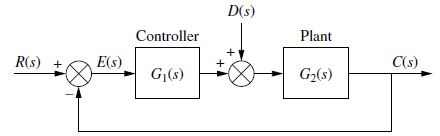
\includegraphics[width=\linewidth]{feedback_control.jpg}
\caption{Feedback Control System with Disturbance}
\end{figure}
\end{center}
%% Reference from p356 of Nise Control Systems textbook
 Presented in the figure above is a simple control system which contains a plant that takes input from a controller, which is driven by an input defined by the reference input R(s) and output C(s); although the laplace notation is used in this figure, R and C could the state vectors of the system. Ignoring the disturbance at this the system in this thesis is virtual, it is known that the gain for this type of system is defined as;

$\frac{C(s)}{R(s)} = \frac{G_1(s) G_2(2)}{ 1 + G_1(s) G_2 (s)}$

and the error is;

$E(s) = \frac{R(s)}{1 + G_1(s) G_2(s)}$

where controllers $G_1(s)$ are designed to minimize $E(s)$,such that the steady-state error is zero;

$e(\infty) = \lim_{s\to0} s * E(s) = 0$

A typical example of a controller has already been mentioned in this paper, and that is the PI (proportional gain plus integral action controller) which was proposed for regulating the servo positions inside a robotic manipulator's joints to a desired joint position. In that circumstance, the controller is defined by the function;

$ G_1 (s) = \frac{K_P s + K_I}{s}$
where $K_P$ and $K_I$ are the proportional and integral gains respectively. In this case, the controller takes in error in servo angle and outputs a voltage that goes to the motor to produce the desired reference on the output. The reason a PI controller is used in this case is due to the integral action's ability to reduce steady state error. This is easily analogous when considering a mechanical system being moved to a desired position. The proportional gain multiplies by the current error to produce a force that moves the system, however there is no judging whether this force is enough to overcome the opposing forces in the system, and may result in an equilibrium position less than that of which is desired. The integral of the error can thus be used, as the error accumulates and gets multiplied by $K_I$, the force grows to overcome the disturbances until the desired location is reached. This can be seen when considering the steady-state error formula with the referenced controller and a mechanical plant with inertial and linear components (thus, at minimum be defined by $[M]s^2 + [K]$);

$ \lim_{s\to0} s * E(s) = s * \frac{R(s)}{1 + \frac{K_P s + K_I}{s} G_2(s)}$

$ \rightarrow e(\infty) = \lim_{s\to0} s   \frac{s   R(s)}{s + (K_P s + K_I) G_2(s)} = \lim_{s\to0} \frac{0}{K_I G_2 (0)} = 0$

Thus integral gain eliminates steady-state error given sufficient time, hence its use as a regulator in servo motors. The use of controllers cannot be mistreated however, as it may have been realised in the mechanical example above, the gains will change the dynamics of the system. Thus, when using controller's it is required that they are tuned to give the desired damping, rise-time and settling time of which is required for the system. In general, the addition of $K_I$ increases overshoot and settling time, which can be counter-acted by the inclusion of a velocity term $K_D$, which for a second order system will decrease overshoot, but incorporate delay into the system. Another negative with using a derivative controller as a regulator in the feed-forward path is that it can lead to over-saturation of the actuator when the reference input is changed between two consequent time samples (step change), producing a 'infinite' gain being multiplied through the plant. The proportional gain is similar to $K_I$, in that if sufficiently large can cause overshoot of the desired position, however, will always result in steady-state error.

This thesis looks into the use of controllers to correct for the error between the desired end-effector position, and the actual. It is proposed that regulating the coordinate space of the end-effector can be achieved by varying the joint angles of the arm with a controller based off the joints' sensitivity in moving the end-effector in a given direction. The premise behind the methodology chosen is backed by the theory presented in this section.\\


%http://www4.cs.umanitoba.ca/~jacky/Robotics/Papers/spong_kinematics.pdf
\section{Forward Kinematics}
As previously mentioned, the forward kinematics of a robotic chain is mathematics that defines the relationship between known joint angles and the end-effect position, such that
$\vec{P} = f( \vec{q} )$ \\
where $\vec{P}$ is the position vector of the end-effector relative to the base of the arm and $\vec{q}$ is a vector of joint angles $\theta_i$ or prismatic joint displacements $d_i$.

This function, $f(\vec{q})$, is found by the translational components of the transformation matrix, $T$, that describes the sequence of twists, rotations and displacements between end-effector position and base of the chain. $T$ can be found by multiplying the transformation between the base link and the next due to $q_1$, by the transformation between the next link and that after due to $q_2$, and so on until the end of the arm, denoted as link number $n$, such that;

$T = A_{0}^i = A_{0}^{1} A_{1}^{2} ... A_{n-1}^n$

The homogenous transformation between two links, $A_{i}^{i+1}$, is created using the product of the rotational transformation about the (rotation axis) z-axis, the translation transform along the z-axis a displacement $d_i$ (the offset in the z-axis from one link to another), the translation transform along the x-axis a displacement $a_i$, and finally the rotational transformation describing the rotation from one x-axis of first joint to the same of the next by an angle denoted $\alpha_i$. These terms are the Denavit-Hartenberg Parameters for the robotic chain, and can be further understood in the figure below provided by Mark W. Spong's Robot Modeling and Control textbook;

\begin{center}
\begin{figure}[htb]
  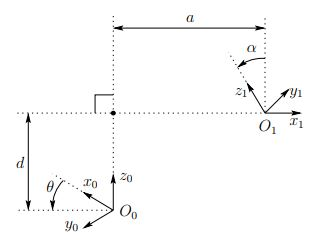
\includegraphics[width=0.5\linewidth]{DH_Parameters_figure.jpg}
\caption{Physical representation of D-H Parameters between two links}
\end{figure}
\end{center}

Where it can be seen that two criteria must be met for the transformation to exist, $z_0$ intersects $x_1$, and axis $x_1$ is perpendicular to axis $z_0$.

\vspace{\baselineskip}
Thus, $A_{i}^{i+1}$ is defined as;

\vspace{\baselineskip}
$A_{i}^{i+i} = Rot_{z,\theta_i} Trans_{z, d_i}, Trans_{x, a_i} Rot_{x, \alpha_i}$

where
\vspace{\baselineskip}
$Rot_{z,\theta_i} =$
$
 \left(\begin{array}{cccc} c_{\theta_i} & -s_{\theta_i} & 0 & 0\\ s_{\theta_i} & c_{\theta_i} & 0 & 0\\ 0 & 0 & 1 & 0\\ 0 & 0 & 0 & 1 \end{array}\right)
$
, 
$Trans_{z, d_i} =$
$
 \left(\begin{array}{cccc} 1 & 0 & 0 & 0\\ 0 & 1 & 0 & 0\\ 0 & 0 & 1 & d_i\\ 0 & 0 & 0 & 1 \end{array}\right)
$

\vspace{\baselineskip}

$Trans_{x, a_i} =$
$
 \left(\begin{array}{cccc} 1 & 0 & 0 & a_i\\ 0 & 1 & 0 & 0\\ 0 & 0 & 1 & 0\\ 0 & 0 & 0 & 1 \end{array}\right)
$
, 
$Rot_{x, \alpha_i} =$
$
 \left(\begin{array}{cccc} 1 & 0 & 0 & 0\\ 0 & c_{\alpha_i} & -s_{\alpha_i} & 0\\ 0 & s_{\alpha_i} & c_{\alpha_i} & 0\\ 0 & 0 & 0 & 1 \end{array}\right)
$
\vspace{\baselineskip}
Thus, the transformation between joints can be described as;
\vspace{\baselineskip}
$A_{i}^{i+1} = $
$ \left(\begin{array}{cccc} c_{\theta_i} & -s{\theta_i} c_{\alpha_i} & s_{\theta_i} s_{\alpha_i} & a_i c_{\theta_i}\\ s_{\theta_i} & c_{\theta_i}c_{\alpha_i} & -c{\theta_i}s{\alpha_i} & a_i s_{\theta_i}\\ 0 & s_{\alpha_i} & c_{\alpha_i} & d_i\\ 0 & 0 & 0 & 1 \end{array}\right)
$
\vspace{\baselineskip}
It can be seen that the homogenous transformation $A_{i}^{i+1}$ contains the 3 dimensional rotation transformation matrix from $i$ to $i+1$, and the column vector representing the translation transformation;
\vspace{\baselineskip}
$A_{i}^{i+1} = $
$ \left(\begin{array}{cccc} & Rot_{i}^{i+1} & & Trans_{i}^{i+1}  \\ 0 & 0 & 0 & 1 \end{array}\right)
$
\vspace{\baselineskip}
Thus, as $T = A_{0}^{1} A_{1}^{2} ... A_{n-1}^n$, $T$ will too have this form. In addition to this, the end-effector position, for arbitrary joint angles $\vec{q}$, can be found by extracting the translational column vector, such that;
\vspace{\baselineskip}
$\vec{P} = f( \vec{q} ) = Trans_{0}^{n} (\vec{q})$

\section{Inverse Kinematics}
The inverse kinematics of a robotic manipulator is the mathematics that defines the angles of the robotic given the position of the end-effector relative to the base of the arm. Using the formula from the previous section, the inverse kinematics can be written as;

$\vec{q} = f^{-1}( \vec{P} )$

Given the derivation from the last section, this computation isn't simple to compute, as the angle vector $\vec{q}$ can contain any number of joint angles, whereas the position vector of the end effector $\vec{P}$ is defined in ${\rm I\!R}^3$. For a 6 joint arm, this gives 6 unknowns and three equations.\\

There are numerous methods that present inverse kinematics solutions to any serial chain of joints; even when there is no known closed form solution. A paper by Gregory Z. Grudic, the University of British Columbia, called Iterative Inverse Kinematics with Manipulator Configuration Control and Proof of Convergence, lists many of the different methods in some detail, including the Tsai and Morgan's solution for a 6 revolute joint arm. \\
%%%%%%%% Need to move this chunk of text to the appendix...
%https://books.google.com.au/books?id=PK_N9aFZ3ccC&printsec=frontcover&dq=tsai+and+morgan+robotics+textbook&hl=en&sa=X&ved=0ahUKEwjRvqqIw63bAhXGwLwKHRxbDAoQ6wEIUjAH#v=onepage&q&f=false
%https://reader.elsevier.com/reader/sd/B3D6C34BEA5F22FD156A30862B225645F137D5CBAEF54030ADE786D00811AE281D632E6381AF7B9758568981C0ABC1B4
Manipulators with 6 rotational joints can reach any position within its stretched length, where motors with more joints are termed as over-actuated robotic actuators and are capable of changing their joint configurations without changing the end-effector position. It is the aforementioned reason that 6 joint robotic arms are of such large interest, and the inverse kinematics is of such high interest.\\
Raghavan and Roth's solution to the inverse kinematics of any 6 joint robotic arm is identified in many research papers and textbooks. It takes the transformations matrices from the forward kinematics, and rearranges them to make a system of equations about joint three. From here, there are 6 unknowns and 5 equations, where by substituting out the trigonometric products form a linear system with 16 unknowns and 6 equations. With more substitutions they arrived at a 12 by 12 matrix written in terms of variables representing trigonometric expressions. The determinant of this matrix gives a 16-degree polynomial referenced to the middle joint, of which can be solved for using a root solver, and the other joint angles found by back substitution. From this, it was concluded that there is 16 possible solutions to the inverse kinematics, however solving a 16-degree polynomial made this method too slow for real-time implementation. The Manocha Method avoids solving the determinant by forming the equations into an eigenvalue problem, where in solving for the eigenvectors gave three of the arm's joint angles with less operations. This was the first real-time inverse kinematics method to be implemented, with methods since being variations of the two outlined above. The Raghavan and Roth method is briefly outlined in appendix C of Lung-Wen Tsai's textbook Robot Analysis: The Mechanics of Serial and Parallel Manipulators. Further, it is worked through along with the Manocha Method in an article from the 14th Triennial World Congress, 1999, A Faster Algorithm for Calculating the Inverse Kinematics of General 6R Manipulator for Robot Real Time Control.\\
It is believed that although new methods derived from those described above form solutions to the inverse kinematics problem in this thesis, as the Jaco arm has 6 revolute joints, the mathematics knowledge and tools for computing the eigenvalues of the complex equations is insufficient.\\


In this thesis, the most common approaches are used to determine the joint angles required to move the Jaco arm's end effector. %Further methods are briefly meantioned and referenced in the inverse kinematics appendix.

\subsection{By Matrix Manipulation Approach}
As previously stated, the transformation that describes the end-effector relative to the base for a set of joint angles can be represented by T such that;
 $T = A_{0}^{1} A_{1}^{2} ... A_{n-1}^n$	eq1
 
From this equation, for a 6 joint arm, it can be determined that;
 
$(A_{0}^{1})^{-1} T = A_{1}^{2} A_{2}^{3} A_{3}^{4} A_{4}^{5} A_{6}^{6}$ eq2

In the Introduction to Robotics: Analysis, Systems, Applications textbook by Saeed B. Niku, it was proposed that mathematical relationships between joints can be found by multiplying both sides of the transformation equation described in eq1, by the inverse transformation between two joints, as seen in eq2. In doing this, it is known that the left hand side must equal the right hand side, however some entries between the left and right may not appear the same, despite being equivalent. From this fact, two entries can be equated together to write trigonometric relationships between joints. It was found that this property is most easily seen where angled twists appear between joints. By iteratively multiplying through by the inverse of a transformation matrix between two joints and inspecting the right and left side's elements, the equations for each joint angle was determined. 

\subsection{Analytical Approach}

A popular approach to solving the inverse kinematics of simple serial chains is by analytically solving the relationship between joints, from the base to the end-effector. This is easiest seen through example, provided by Lung-Wen Tsai's Robot Analysis textbook.

\begin{center}
\begin{figure}[htb]
  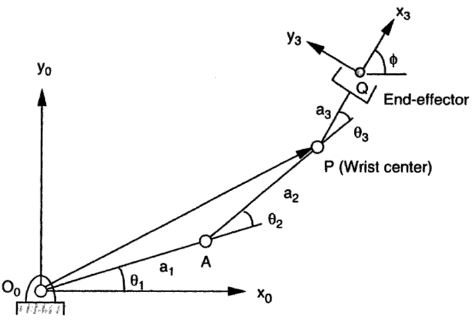
\includegraphics[width=0.8\linewidth]{Tsai_3rr.jpg}
\caption{Revolute Joint Arm}
\end{figure}
\end{center}

It can be seen in the figure above, that the end-effector is described by the coordinate vector $\vec{Q}$, with a joint 3 being represented in space by vector $\vec{P}$. It can also be seen that lengths $a_1$ and $a_2$ form a triangle with vector $\vec{P}$, dependent on the varying angles of $\theta_1$ and $\theta_2$. In addition to this, it can be seen that the four equations can be derived between the points;

$p_x = a_1 c\theta_1 + a_2 c \theta_{12}$\\
$p_y = a_1 s\theta_1 + a_2 s \theta_{12}$\\
$p_x = q_x - a_3 c\sigma$\\
$p_y = q_y - a_3 s\sigma$\\

where $\sigma = \theta_1 + \theta_2 + \theta_3$

From the cosine rule, the triangle can be defined by;

$p_x^2 + p_y^2 = a_1^2 + a_2^2 + 2 a_1 a_2 c \theta_2$

which can be rearranged for $\theta_2$ in terms of point P and the arm lengths such that;

$\theta_2 = cos^{-1} ( \frac{p_x^2 + p_y^2 - a_1^2 - a_2^2 }{2 a_1 a_2} )$
which will have two solutions depending on the evaluation of the fraction within the inverse cosine, and the arm is fully stretched when this equates to 1.

The equations describing $p_x, p_y$ in terms of $\theta_1, \theta_2$ above can be rearranged for $cos(\theta_1), sin(\theta_1)$ such that;

$c \theta_1 = \frac{p_x (a_1 + a_2 c \theta_2 ) + p_y a_2 s \theta_2}{a_1^2 + a_2^2 + 2 a_1 a_2 c \theta_2}$

$s \theta_1 = \frac{p_y (a_1 + a_2 c \theta_2 ) - p_x a_2 s \theta_2}{a_1^2 + a_2^2 + 2 a_1 a_2 c \theta_2}$

and $\theta_1$ can be computed by;

$\theta_1 = Atan2(s\theta_1, c\theta_1)$

Using the desired end-effector position Q, the third angle can thus be solved from its relationship to point P, described above. This method can be repeated working up the joints, were the position of each link can give the required joint angles. The equations outlined in this section were used in the final product of this thesis.


% what is the jacobian!?!?!?!
\subsection{Jacobian}
The Jacobian is a linearised representation of the dynamics of a system for a particular set of states. For example, the system for a robotic arm can be computed by Lagrange Equations, to have the form;

$[\tau] = [M(q)] \ddot{q} + [ C (q, \dot{q} ) ] \dot{q} + [G(q)]$

Where $\tau$ is a vector of the applied joint torques, $q$ describes the joint angles such that $\dot{q}$ is the joint velocity vector and $\ddot{q}$ is the joint acceleration vector. As the arm moves, the perpendicular distance to gravity from the arm's base each joint will vary, and thus so will the torque due to gravity; this dynamics is covered in the matrix $G$, which depends on $q$. The matrix C contains the Coriolis and centripetal terms that make up the gyroscopic torques experienced as the arm swings around, which is a function of velocity and angle. Finally, the matrix M represents the torques experienced due to the inertia of the arm's links, which is a function of joint accelerations, and varies with joint angles.\\
One is able to control the arm using a supplied torque once these dynamics are known, however for a 6 DOF arm, there will be 60 parameters that need to be found to accurately described the motion. By taking the Taylor Series expansion of the equation of motion described above, about a linearised set of joint angles, the small change in angles required for a change in end-effector position can be determined; it is this matrix result that is termed the Jacobian. This can be described below, where $\vec{X}$ represents the change in end-effector position. Where $\tau$ is described by the equation above, the force $F$ of the end effector for a small change in end-effector position, can be used to find the change in angles;

$\tau \delta \vec{q} = F \delta	\vec{X}$

$\tau = J^T F$

An alternative approach to using the dynamics of the system to compute the Jacobian matrix, it to derive it from the forward kinematics transformation matrix; which already describes a relationship between joint angles and end effector position. 

From the transformation matrix, it was found that the position of the end effector $\vec{P}$ can be found by;

$\vec{P} = f( \vec{q} )$

The problem came when considering the inverse of $f(\vec{q})$, which is a 3x6 matrix for a 6 joint arm; as this matrix is rank deficient it cannot be inverted. Three more states that describe the position of the end-effector is required to construct a square matrix, and these are the end-effector's angular positions relative to the base of the arm, as described by the rotation matrix within the transformation matrix $T$.

From the transformation matrix, it can be seen that a small change in angle $q_i$ can cause a small change in rotation and translation of the end effector such that;

$\frac{\delta T}{\delta q_i} = $
$ \left(\begin{array}{cccc} & \frac{\delta R}{\delta q_i} & & \frac{\delta t}{\delta q_1}  \\ 0 & 0 & 0 & 0 \end{array}\right)
$

In three dimensions, angular velocity can be represented by the Skew matrix;

$S(\omega) = $
$ \left(\begin{array}{ccc} 0 & -\omega_z & \omega_y \\ \omega_z & 0 & -\omega_x  \\ -\omega_y & \omega_x & 0 \end{array}\right)
$

Thus, the angular velocity vector $(\omega_x, \omega_y \omega_z)^T$ can be found from forming the Skew matrix such that;

$S(\omega) = \frac{\delta R}{\delta q_i} R^T \dot{q_i}$

by equating coefficients.\\

From this, the Jacobian for a 6 DOF arm can be described as;

$J = $
$ \left(\begin{array}{cccccc} 
\frac{\delta x}{\delta q_1} & \frac{\delta x}{\delta q_2} & \frac{\delta x}{\delta q_3} & \frac{\delta x}{\delta q_4} & \frac{\delta x}{\delta q_5} & \frac{\delta x}{\delta q_6} \\ 
\frac{\delta y}{\delta q_1} & \frac{\delta y}{\delta q_2} & \frac{\delta y}{\delta q_3} & \frac{\delta y}{\delta q_4} & \frac{\delta y}{\delta q_5} & \frac{\delta y}{\delta q_6} \\ 
\frac{\delta z}{\delta q_1} & \frac{\delta z}{\delta q_2} & \frac{\delta z}{\delta q_3} & \frac{\delta z}{\delta q_4} & \frac{\delta z}{\delta q_5} & \frac{\delta z}{\delta q_6} \\ 
\frac{\delta \theta_x}{\delta q_1} & \frac{\delta \theta_x}{\delta q_2} & \frac{\delta \theta_x}{\delta q_3} & \frac{\delta \theta_x}{\delta q_4} & \frac{\delta \theta_x}{\delta q_5} & \frac{\delta \theta_x}{\delta q_6} \\ 
\frac{\delta \theta_y}{\delta q_1} & \frac{\delta \theta_y}{\delta q_2} & \frac{\delta \theta_y}{\delta q_3} & \frac{\delta \theta_y}{\delta q_4} & \frac{\delta \theta_y}{\delta q_5} & \frac{\delta \theta_y}{\delta q_6} \\ 
\frac{\delta \theta_z}{\delta q_1} & \frac{\delta \theta_z}{\delta q_2} & \frac{\delta \theta_z}{\delta q_3} & \frac{\delta \theta_z}{\delta q_4} & \frac{\delta \theta_z}{\delta q_5} & \frac{\delta \theta_z}{\delta q_6} 
\end{array}\right)
$

Thus, the change in end-effector position that results from a change of angles is;

$\frac{dX}{dt} = J \frac{dq}{dt}$

and the change in angles required for a change in end-effector position;

$\frac{dq}{dt} = J^{-1} \frac{dX}{dt}$

In the case that the Jacobian isn't invertible the Pseudo Inverse Jacobian can be used; when one of the angular velocities doesn't change with angle, which occurs when there are less than 6 DOF in the arm. Thus, the objective of this method is to make the Jacobian full rank, by multiplying the Jacobian by its transpose, resulting in;

$\frac{dq}{dt} = J^T (J J^T)^{-1} \frac{dX}{dt} $

\subsection{Damped Least Squares}
%http://graphics.cs.cmu.edu/nsp/course/15464-s17/lectures/iksurvey.pdf
The damped least squares method provides a more stable set of change in angles required for small errors in end-effector position close to arm singularities, however takes longer to compute. This method looks to minimize this error by the following quantity;

$\Delta \theta = (J^T J + \lambda^2 I)^{-1} J^T \Delta X$

given a non-zero damping constant $\lambda$. There are numerous methods for finding a good quantity for $\lambda$, however in general it should be large enough such that the solution is stable near singularities, but not too large or else accuracy is reduced.

% feedback loop of error that interally creates a better approximation
%https://www.coursera.org/learn/modernrobotics-course2/lecture/EBBuh/numerical-inverse-kinematics-chapter-6-2-part-1-of-2
%http://www.math.ubc.ca/~anstee/math104/newtonmethod.pdf
%http://old.cescg.org/CESCG-2002/LBarinka/paper.pdf
%http://graphics.cs.cmu.edu/nsp/course/15464-s17/lectures/iksurvey.pdf
\subsection{Newton-Raphson Method}
The Newton-Raphson method is a numerical methods technique on homing-down on a better approximation than one given. It was found that, once an approximation gives a result with small error from the expected, a better solution can be made by reusing formula with the result of the original guess, where convergence on an accurate solution can be retrieved given enough iterations in the local space to the original guess.

from the Taylor's expansion, it is known thatthe true position x can be given by a previous position $x_0$ plus $h$, for small changes in position $h$, ;

$f(x) = f(x_0 + h) \approx f(x_0) + h f'(x_0)$

and thus;

$h \approx - \frac{f(x_0)}{f'(x_0)}$

therefore, the true position can be approximated by;

$x = x_0 + h \approx x+0 - \frac{f(x_0)}{f'(x_0)}$

using this property in iteration, the true position x will be converged on, such that the next estimate for iteration number $n$ is given by;

$x_{n+1} = x_n - \frac{f(x_n)}{f'(x_n)}$

It has already been described that the Jacobian can be used to approximate the change in joint angles required for a change in end-effector position, thus, a better approximation of these angles can be determined using the Newton-Raphson method. Given a the Taylors expansion of a desired end-effector position $x_d$;

$x_d = f( \theta _d ) = f( \theta ^k ) + \frac{ \Delta f }{ \Delta \theta } |_{ \theta ^k } ( \theta_d - \theta^k ) + ( higher\ order\ terms )$

it is known that

$J(\theta^k) = \frac{\Delta f}{\Delta \theta} |_{\theta^k}$

and

$\Delta \theta = (\theta_d - \theta^k)$

This gives;

$x_d - f(\theta^k) = J(\theta^k) \Delta \theta$

$\Delta X = J(\theta^k) \Delta \theta$

Thus, this matches the form used in the Newton-Raphson method, and the iteration method can be used to create a better approximation of $\Delta X$ given a better approximation of $\Delta \theta$. This process is described in the figure below;

\begin{center}
\begin{figure}[htb]
  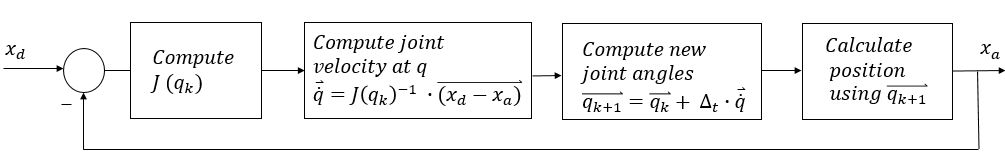
\includegraphics[width=\linewidth]{Newton-Raphson_loop.jpg}
\caption{The Newton-Raphson Method applied to Inverse Kinematics}
\end{figure}
\end{center}

V-REP uses this approach for its inverse kinematics solver; except with the Pseudo-Inverse Jacobian, as it intrinsically provides the smallest 2-norm among all solutions, even when the arm is near singularities. When a set of joints is in inverse kinematics mode, either the Pseudo Inverse or Damped Least Squares method can be chosen, with an iteration number. This iteration number is the number of times V-REP will perform the above loop before using the evaluated change in angles to move the joints. Thus, the number of iterations determines the accuracy of these methods, where the more iterations the more processing time is required to narrow down on a more accurate solution.

\begin{center}
\begin{figure}[htb]
  \includegraphics[width=0.5\linewidth]{VREP_ik_dialog.jpg}
\caption{The calculation method for Inverse Kinematics in V-REP}
\end{figure}
\end{center}

Due to V-REP's knowledge on the position of joints within a serial chain, using the inbuilt D-H solver the transformation matrix for the arm is determined. Thus, from this the Jacobian, and then the Pseudo-Jacobian matrices are computed for a given configuration, and used to calculate the change in angles required for the `Tip` object to reach the `Target` object; given a solver type as specified above. This method will be mimicked in this thesis such that the client program can have the ability to control the joint angles of both V-REP and the physical Kinova Jaco arm.

\chapter{Design Approach}

This chapter looks into the design of the client program, the decisions and functionality required to complete the program's objectives. Firstly the overall objectives are defined, and then the procedures for completing these are provided. The results chapter will go into detail of how the functionality was implemented, and the successes and failures which arose.

\section{Client Program Functionality Requirements and Design}
Using V-REP's remote API, a client program is required to be developed to allow the external control of the virtual Jaco arm. This program must have the following functionality:

\begin{itemize}
	\item Be able to control a scene with the Jaco arm with joints either in Forward or Inverse Kinematics modes
	\item Allow input commands come from the user's keyboard, or from an external joystick
	\item Allow the control of the Jaco arm by calculating its own inverse kinematics
	\item Be able to connect to V-REP through a specified IP address and port number
	\item Be easily able to convert between implemented kinematics modes
	\item Have data-steaming functionality to enable collision detection
	\item Be able to quickly retrieve the object handles for the joints of the Jaco arm, for any given V-REP scene before processing
	\item Be able to identify when the Jaco arm is in an undesirable configuration and have automatic adjustments; an undesirable configuration is when the gripper is facing upwards, as if to grab something from above, instead of out in front.
	\item Allow real-time manipulation of the virtual robotic arm and V-REP scene
\end{itemize}


Considering there was a distinct lack of background experience with V-REP and using remote API's, the development of the client program was broken down into small stages. These stages together allowed the full development of the program:

\begin{enumerate}
  \item 
  \item 
\end{enumerate}



\section{Client Program Approach}






\chapter{Methodology, procedure, design, etc.}

This may be one chapter or several.  Again, titles should be more
informative than the above.

You will almost certainly need diagrams to clarify your meaning.  The
\LaTeXe\ \texttt{graphics} package allows the inclusion of PostScript
graphics, as in \fig{flr1}.  The inclusion of \LaTeX\ \texttt{picture}
graphics, as in \fig{fzsys}, requires no auxiliary packages and allows
the mathematical formatting features of \LaTeX\ to be used in
diagrams; but the \texttt{picture} files, unlike PostScript files,
usually require manual editing.





\chapter{Results and discussion \ldots}

\ldots\ or perhaps the discussion should be a separate chapter.

In any case, you will probably need to include tabulated results.
\tab{tf2} illustrates the use of various \LaTeX\ environments to
include a computer printout (plain text file) in a document.  The
\texttt{verbatim} environment, which encloses the formatted text, is
also useful for program listings.

\begin{table}\renewcommand{\baselinestretch}{1.0}
\caption{\sl Fraction of air volume involved in heat exchange for
second mode (right column) vs.\ filling factor (left column).  The
plain-text headings represent $f$, $m$, $\mu_2$ and $f_2$.}
\label{tf2}

\begin{center}
\begin{minipage}[c]{2.85in}\small\normalsize
\begin{verbatim}

 f(%)     m         mu2     f2(%)

 0.016   80.00    0.05400   4.874
 0.031   56.57    0.07732   5.438
 0.062   40.00    0.11103   6.125
 0.125   28.28    0.16001   6.970
 0.250   20.00    0.23175   8.020
 0.500   14.14    0.33799   9.329
 1.000   10.00    0.49789  10.967
 2.000    7.07    0.74444  13.008
 4.000    5.00    1.13919  15.525
 8.000    3.54    1.81095  18.568

19.237    2.28    3.61958  23.174
37.180    1.64    7.28635  27.094
57.392    1.32   14.63631  29.813
74.316    1.16   29.35160  31.453
85.734    1.08   58.79364  32.360
\end{verbatim}
\end{minipage}
\end{center}
\end{table}

\chapter{Conclusions}

\section{Summary and conclusions}

\section{Possible future work}

\appendix

% Chapters after the \appendix command are lettered, not numbered.
% Setting apart the appendices in the table of contents is awkward:

\newpage
\addcontentsline{toc}{part}{Appendices}
\mbox{}
\newpage

% The \mbox{} command between two \newpage commands gives a blank page.
% In the contents, the ``Appendices'' heading is shown as being on this
% blank page, which is the page before the first appendix.  This stops the
% first appendix from be listed ABOVE the word ``Appendices'' in the
% table of contents.

% \include appendix chapters here.

\chapter{Dummy appendix}

Appendices are useful for supplying necessary details or explanations
which do not seem to fit into the main text, perhaps because they are
too long and would distract the reader from the central argument.
Appendices are also used for program listings.

Notice that appendices are ``numbered'' with capital letters, not
numerals.  When the \verb+\appendix+ command in
\LaTeX~\cite[p.\,175]{lamport} is used with the \texttt{book} document
class, it causes subsequent chapters to be treated as appendices.

\chapter{Program listings}

\section{First program}

Some initial explanatory notes may precede the listing.

\section{Second program}

\section{Etc.}

\chapter{Companion disk}

If you wish to make some computer files available to your examiners,
you can list and describe the files here.  The files can be supplied
on a disk and inserted in a pocket fixed to the inside back cover.

The disk will not be needed if you can specify a URL from which the
files can be downloaded.

\cleardoublepage

\begin{thebibliography}{99}
\addcontentsline{toc}{chapter}{Bibliography}
\bibitem{lamport} L.~Lamport, \emph{\LaTeX: A Document Preparation
System}, 2nd ed. (Addison-Wesley, 1994).
\bibitem{LABEL2} REFERENCE 2
\bibitem{ETC.} Etc.
\end{thebibliography}

\end{document}